% Standalone pages of the architecture figures used in the GitHub release (one figure per page).
%   pdflatex release_figures.tex  ->  pdftoppm -png -r 220 release_figures.pdf fig
\documentclass[border=10pt,tikz]{standalone}
\usepackage{amsmath,amssymb,bm}
\usepackage[obeyspaces,spaces]{url}
\usetikzlibrary{arrows.meta,positioning,fit,backgrounds,calc}
\newcommand{\T}{^{\mathsf T}}
\newcommand{\sat}{\operatorname{sat}}
\newcommand{\clip}{\operatorname{sat}}   % manuscript notation (2026-10-01): sat for every interval limit
\newcommand{\sgnp}{\operatorname{sgn}_{+}}
\newcommand{\code}[1]{\path{#1}}
\newcommand{\Peq}[1]{P-(#1)}
\renewcommand{\ref}[1]{1}
\newif\ifwithbs \withbsfalse          % the recursive-backstepping extension stays out of the release
% Shared TikZ style for all architecture figures. Grayscale-safe.
\tikzset{
  blk/.style   ={draw,rounded corners=2pt,align=center,font=\footnotesize,
                 minimum height=8mm,inner sep=3pt,fill=white},
  clas/.style  ={blk,fill=black!4},
  neuro/.style ={blk,fill=black!12,very thick},
  plant/.style ={blk,fill=black!20},
  meas/.style  ={blk,dashed},
  sum/.style   ={draw,circle,inner sep=0pt,minimum size=4.5mm,font=\scriptsize},
  sig/.style   ={-{Latex[length=2mm]},thick},
  sigd/.style  ={-{Latex[length=2mm]},thick,dashed},
  lbl/.style   ={font=\scriptsize,inner sep=1.5pt,fill=white},
  grp/.style   ={draw,dashed,rounded corners=3pt,inner sep=6pt},
  note/.style   ={font=\scriptsize\itshape,align=left},
}

% Extra styles for the controller-family figures; the base styles (blk, clas, neuro, plant, sig, ...) are the
% manuscript's own architectures/tikz/arch_style.tex, so every figure matches the paper's Fig. 1.
\tikzset{
  law/.style    ={blk,fill=blue!7,draw=blue!45!black,thick},
  offl/.style   ={blk,dashed,fill=black!2},
  fam/.style    ={draw=blue!45!black,dashed,rounded corners=3pt,inner sep=7pt},
  famlbl/.style ={font=\scriptsize\itshape,text=blue!45!black,inner sep=1pt},
  off/.style    ={-{Latex[length=2mm]},thick,dotted,gray},
  every node/.append style={font=\footnotesize},
}
% Common left half: reference generator and attitude error (identical for every family).
\newcommand{\commonleft}{%
  \node[clas] (ref) at (0,0) {\textbf{Mission reference}\\$q_d(t)$\\[1pt]
        $\bm\omega_d$: central difference};
  \node[clas,right=7mm of ref] (err) {\textbf{Attitude error}\\$q_e=q_d\otimes q^{-1}$\\
        $\bm e=2\,\sgnp(q_{e,0})\,\bm q_{e,v}$\\$\bm\omega_e=\bm\omega-\bm\omega_d$};
  \draw[sig] (ref) -- node[lbl,above]{$q_d,\bm\omega_d$} (err);
}
% Common right half and feedback of every family figure. Needs nodes (err) and (law-out) placed by the figure,
% and the coordinate (satx) giving the x position of the torque box.
\newcommand{\commonloop}[2]{% #1: label on u0 arrow source node, #2: text inside the torque-box node
  \node[clas] (sat) at (satx) {#2};
  \node[neuro,below=13mm of sat] (res) {\textbf{Gated CMG--PES residual}\\(Fig.~\ref{fig:interface})\\
        $\bm u=\sat_{\bm\ell}(\bm u_0+\beta\bm\ell\odot\tilde{\bm s})$};
  \node[plant,anchor=east] (plant) at ($(res.west)+(-12mm,0)$) {\textbf{Allocation and MuJoCo plant}\\
        $\bm f=\clip_{[\bm0,\bm f_{\max}]}(B^{-1}[T,\bm u\T]\T)$\\X2 / CF2 rigid body};
  \draw[sig] (#1) -- (sat);
  \draw[sig] (sat) -- node[lbl,right]{$\bm u_0\in\mathcal U$} (res);
  \draw[sig] (res) -- node[lbl,above]{$\bm u$} (plant);
  \draw[sig] (plant.west) -- ++(-4mm,0) coordinate (fb1) -| node[lbl,pos=.75,left]{measured $q,\ \bm\omega$} (err.south);
}

\begin{document}
% 1 CMG unit coupling topology (paper Fig. 2)
% B1c -- column-native CMG unit: coupling topology only. The state
% equations stay in the text; the figure shows which variable acts on which.
% Natural width is about one IEEE column, so no \resizebox is needed.
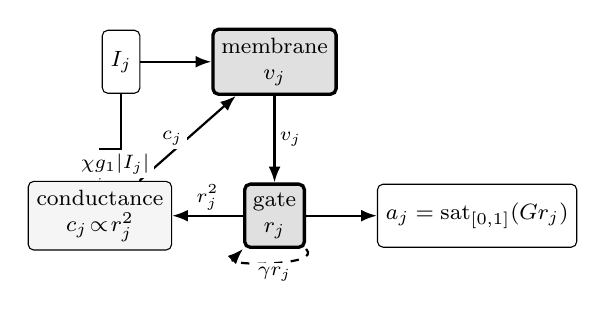
\begin{tikzpicture}[node distance=6mm and 9mm,font=\footnotesize]
  \node[blk]                       (I) {$I_j$};
  \node[neuro,right=of I]          (v) {membrane\\$v_j$};
  \node[neuro,below=11mm of v]     (r) {gate\\$r_j$};
  \node[clas,left=of r]            (c) {conductance\\$c_j\!\propto\! r_j^{2}$};
  \node[blk,right=of r]            (a) {$a_j=\clip_{[0,1]}(G r_j)$};

  \draw[sig] (I) -- (v);
  \draw[sig] (v.south) -- node[lbl,right]{$v_j$} (r.north);
  \draw[sig] (r) -- node[lbl,above]{$r_j^{2}$} (c);
  \draw[sig] (c) -- node[lbl,left]{$c_j$} (v);
  \draw[sig] (r) -- (a);
  \draw[sigd] (r.south east) to[out=-45,in=-135]
        node[lbl,below]{$\gamma r_j$} (r.south west);
  \draw[sig] (I.south) -- ++(0,-7mm) -| node[lbl,pos=.14,below]{$\chi g_1|I_j|$} (c.north);
\end{tikzpicture}

% 2-9 controller families
% How every family attaches to the same gated CMG--PES residual (Sec. 2). Row 1: the six u0 sources and the
% plant path; rows 2-3: the residual path of the manuscript's Fig. 1, unchanged.
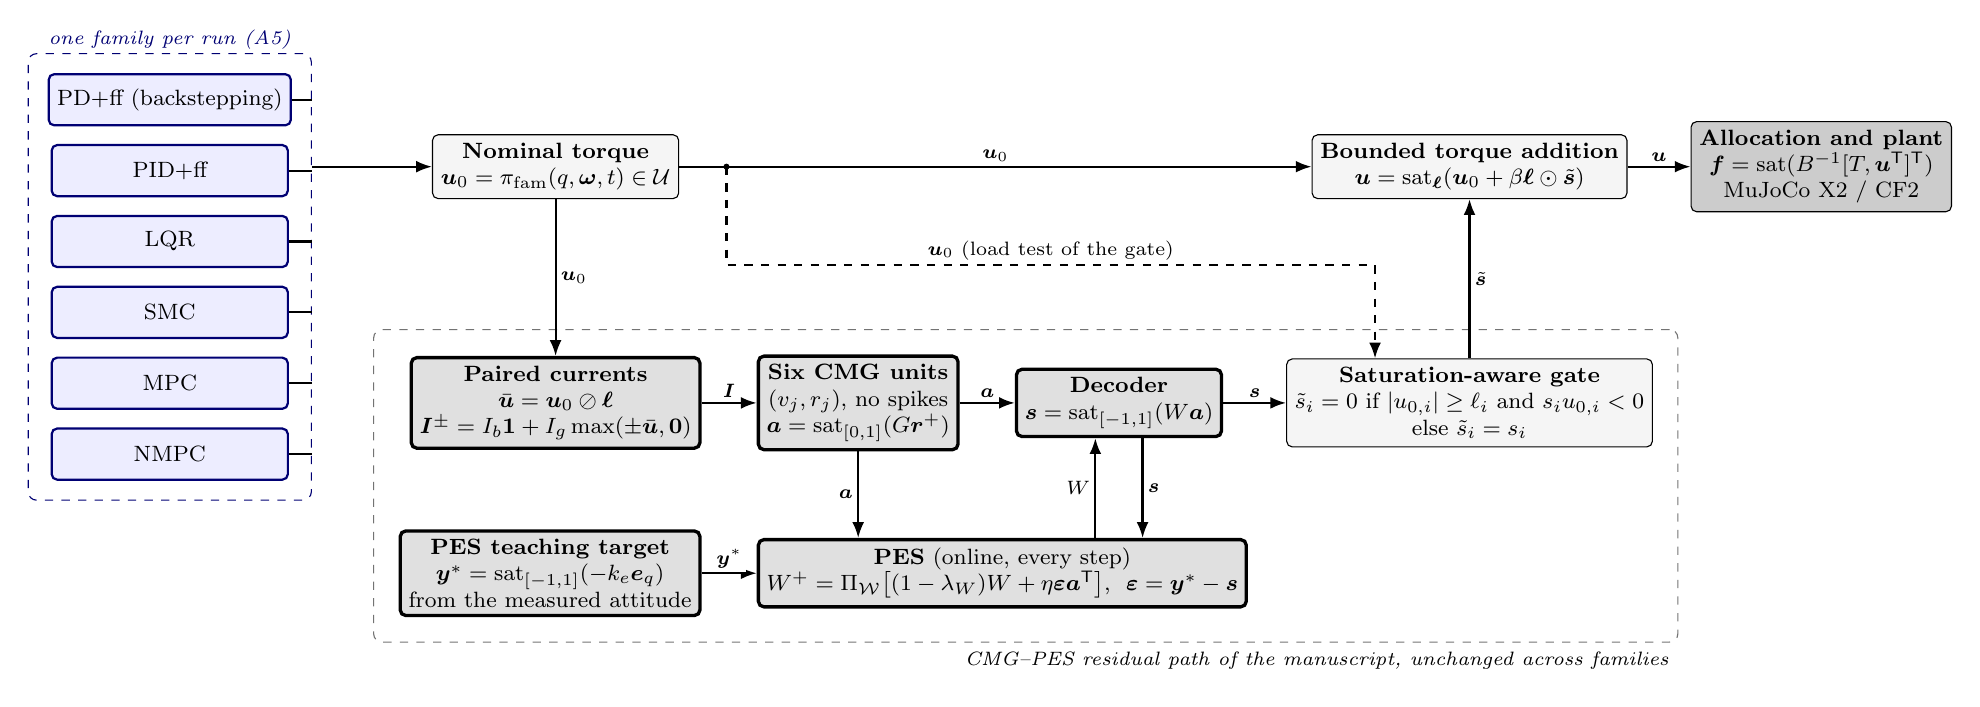
\begin{tikzpicture}
  % ---- six u0 sources -----------------------------------------------------------------------------------------
  \foreach \n/\t [count=\i] in {f1/PD+ff (backstepping),f2/PID+ff,f3/LQR,f4/SMC,f5/MPC,f6/NMPC}
    \node[law,minimum height=6.5mm,minimum width=30mm] (\n) at (0,{1.75-0.9*\i}) {\t};
  \ifwithbs
  \node[law,dashed,minimum height=6.5mm,minimum width=30mm,align=center] (f7) at (0,{1.75-0.9*7-0.25}) {Recursive backstepping\\(new, not in paper)};
  \node[fam,fit=(f1)(f7)] (fams) {};
  \else
  \node[fam,fit=(f1)(f6)] (fams) {};
  \fi
  \node[famlbl,anchor=south] at (fams.north) {one family per run (A5)};
  \ifwithbs\def\nfam{7}\else\def\nfam{6}\fi
  \foreach \i in {1,...,\nfam} \draw[thick] (f\i.east) -- (f\i.east-|fams.east);

  % ---- residual path (manuscript Fig. 1) -----------------------------------------------------------------------
  \node[neuro] (enc)  at (4.9,-3.0) {\textbf{Paired currents}\\$\bar{\bm u}=\bm u_0\oslash\bm\ell$\\
        $\bm I^\pm=I_b\bm1+I_g\max(\pm\bar{\bm u},\bm0)$};
  \node[neuro] (cmg)  [right=7mm of enc] {\textbf{Six CMG units}\\$(v_j,r_j)$, no spikes\\$\bm a=\clip_{[0,1]}(G\bm r^+)$};
  \node[neuro] (dec)  [right=7mm of cmg] {\textbf{Decoder}\\$\bm s=\clip_{[-1,1]}(W\bm a)$};
  \node[clas]  (gate) [right=8mm of dec] {\textbf{Saturation-aware gate}\\$\tilde s_i=0$ if $|u_{0,i}|\ge\ell_i$ and $s_iu_{0,i}<0$\\
        else $\tilde s_i=s_i$};
  \node[neuro] (pes)  [below=11mm of cmg.south west,anchor=north west] {\textbf{PES} (online, every step)\\
        $W^+=\Pi_{\mathcal W}\big[(1-\lambda_W)W+\eta\bm\varepsilon\bm a\T\big]$,\ \ $\bm\varepsilon=\bm y^*-\bm s$};
  \node[neuro] (tgt)  [left=7mm of pes] {\textbf{PES teaching target}\\$\bm y^*=\clip_{[-1,1]}(-k_e\bm e_q)$\\from the measured attitude};

  % ---- plant path ----------------------------------------------------------------------------------------------
  \node[clas]  (sel)   at (enc|-0,0) {\textbf{Nominal torque}\\$\bm u_0=\pi_{\rm fam}(q,\bm\omega,t)\in\mathcal U$};
  \node[clas]  (box)   at (gate|-0,0) {\textbf{Bounded torque addition}\\$\bm u=\sat_{\bm\ell}(\bm u_0+\beta\bm\ell\odot\tilde{\bm s})$};
  \node[plant] (plant) [right=8mm of box] {\textbf{Allocation and plant}\\$\bm f=\clip(B^{-1}[T,\bm u\T]\T)$\\MuJoCo X2 / CF2};
  \draw[sig] (fams.east|-sel) -- (sel);
  \draw[sig] (sel) -- node[lbl,above]{$\bm u_0$} (box);
  \draw[sig] (box) -- node[lbl,above]{$\bm u$} (plant);

  % ---- signals ---------------------------------------------------------------------------------------------------
  \draw[sig] (sel) -- node[lbl,right]{$\bm u_0$} (enc);
  \draw[sig] (enc) -- node[lbl,above]{$\bm I$} (cmg);
  \draw[sig] (cmg) -- node[lbl,above]{$\bm a$} (dec);
  \draw[sig] (dec) -- node[lbl,above]{$\bm s$} (gate);
  \draw[sig] (gate) -- node[lbl,right]{$\tilde{\bm s}$} (box);
  \draw[sig] (cmg.south) -- node[lbl,left]{$\bm a$} (cmg.south|-pes.north);
  \draw[sig] ($(pes.north-|dec)+(-3mm,0)$) -- node[lbl,left]{$W$} ($(dec.south)+(-3mm,0)$);
  \draw[sig] ($(dec.south)+(3mm,0)$) -- node[lbl,right]{$\bm s$} ($(pes.north-|dec)+(3mm,0)$);
  \draw[sig] (tgt) -- node[lbl,above]{$\bm y^*$} (pes);
  \coordinate (u0tap) at ($(sel.east)+(6mm,0)$);
  \fill (u0tap) circle (1.1pt);
  \draw[sigd] (u0tap) -- ++(0,-1.25) -| node[lbl,pos=.25,above]{$\bm u_0$ (load test of the gate)} ($(gate.north)+(-12mm,0)$);

  \begin{scope}[on background layer]
    \node[fam,draw=black!55,fit=(enc)(cmg)(dec)(gate)(pes)(tgt),inner sep=9pt] (rp) {};
  \end{scope}
  \node[note,anchor=north east] at (rp.south east) {CMG--PES residual path of the manuscript, unchanged across families};
\end{tikzpicture}

% PD+ff in backstepping (computed-torque) form: the paper's rho = 3 primary baseline.
\begin{tikzpicture}
  \commonleft
  \node[law,right=10mm of err] (law) {\textbf{Computed-torque backstepping}\\
        $\bm a=\dot{\bm\omega}_d-k_1\bm e-k_2\bm\omega_e$\\$k_1=(\rho\omega_n)^2,\quad k_2=2\zeta\rho\omega_n$};
  \node[offl,above=9mm of law] (ff) {\textbf{Model feedforward} (off in every run)\\
        $\bm J\odot\dot{\bm\omega}_d$ \ and \ $\bm\omega\times(\bm J\odot\bm\omega)$};
  \draw[off] (ff) -- node[lbl,right]{$\times0$} (law);
  \draw[sig] (err) -- node[lbl,above]{$\bm e,\bm\omega_e$} (law);
  \coordinate (satx) at ($(law.east)+(25mm,0)$);
  \commonloop{law}{\textbf{Torque box}\\$\bm u_0=\sat_{\bm\ell}(\bm J\odot\bm a)$};
  \node[fam,fit=(law)(ff)] (g) {};
  \node[famlbl,anchor=south west] at (g.north west) {family: PD+ff, backstepping form (\code{--baseline backstepping})};
\end{tikzpicture}

% PID+ff with conditional-integration anti-windup at rotor level (run_controllers_gated.py, --baseline pd).
\begin{tikzpicture}
  \commonleft
  \node[law,right=12mm of err] (law) {\textbf{PID + rate feedforward}\\
        $\bm\tau_{\rm u}=-\bm k_q\odot\bm e_q-\bm k_\omega\odot\bm\omega_e-\bm k_i\odot\bm z$\\
        $\bm k_q=2\bm J\odot\bm\omega^2,\ \bm k_\omega=2\zeta\bm J\odot\bm\omega,\ \bm k_i=0.3\bm k_q$,\ \ $\bm\omega=\rho\bm\omega_n$};
  \node[law,above=12mm of law] (int) {\textbf{Conditional integrator}\\
        $z_i^+=z_i+h\,e_{q,i}\,m_i$\\
        $m_i=1$ iff axis $i$ was not clipped \emph{and}\\no rotor saturated at the previous step};
  \draw[sig] (int) -- node[lbl,right]{$\bm z$} (law);
  \draw[sig] (err) -- node[lbl,above]{$\bm e_q,\bm\omega_e$} (law);
  \draw[sig] ($(err.north)+(4mm,0)$) |- node[lbl,pos=.75,above]{$\bm e_q$} ($(int.west)+(0,2mm)$);
  \coordinate (satx) at ($(law.east)+(24mm,0)$);
  \commonloop{law}{\textbf{Torque box}\\$\bm u_0=\sat_{\bm\ell}(\bm\tau_{\rm u})$};
  \draw[sigd] (sat.north) |- node[lbl,pos=.3,right]{clip active on axis $i$?} (int.east);
  \draw[sigd] ($(plant.north)+(-10mm,0)$) -- ($(plant.north)+(-10mm,4mm)$) -| ($(law.west)+(-5mm,0)$)
        |- ($(int.west)+(0,-3mm)$);
  \node[lbl,anchor=east,align=right] at ($(law.north west)+(-6mm,5mm)$) {rotor saturated\\at step $k-1$};
  \node[fam,fit=(law)(int)] (g) {};
  \node[famlbl,anchor=south west] at (g.north west) {family: PID+ff (\code{--baseline pd --ki-factor 0.3 --antiwindup rotor})};
\end{tikzpicture}

% LQR: per-axis double integrator, closed-form CARE gain.
\begin{tikzpicture}
  \commonleft
  \node[law,right=10mm of err] (law) {\textbf{LQR state feedback} (per axis)\\
        $a_i=\dot\omega_{d,i}-K_i\,[e_i,\ \omega_{e,i}]\T$\\$K_i=[\omega_i^2,\ \sqrt2\,\omega_i]$,\ \ $\omega_i=\rho\omega_{n,i}$};
  \node[offl,above=9mm of law] (care) {\textbf{CARE, solved in closed form}\\
        $\dot{\bm x}=\left[\begin{smallmatrix}0&1\\0&0\end{smallmatrix}\right]\bm x+\left[\begin{smallmatrix}0\\1\end{smallmatrix}\right]a$,\ \
        $\bm x=[e,\omega_e]\T$\\$Q=\operatorname{diag}(\omega^4,0)$,\ \ $R=1$};
  \draw[sigd] (care) -- node[lbl,right]{$K$ (fixed)} (law);
  \draw[sig] (err) -- node[lbl,above]{$\bm e,\bm\omega_e$} (law);
  \coordinate (satx) at ($(law.east)+(25mm,0)$);
  \commonloop{law}{\textbf{Torque box}\\$\bm u_0=\sat_{\bm\ell}(\bm J\odot\bm a)$};
  \node[fam,fit=(law)(care)] (g) {};
  \node[famlbl,anchor=south west] at (g.north west) {family: LQR (\code{--baseline lqr})};
\end{tikzpicture}

% SMC: linear sliding variable, boundary-layer reaching law.
\begin{tikzpicture}
  \commonleft
  \node[law,right=10mm of err] (law) {\textbf{Boundary-layer reaching law}\\
        $\bm a=\dot{\bm\omega}_d-\lambda\bm\omega_e-\bm\eta\odot\sat(\bm\sigma\oslash\bm\phi)$\\
        $\bm\eta=0.5\,\bm\ell\oslash\bm J$,\quad $\bm\phi=\bm\eta\oslash\lambda$};
  \node[law,above=9mm of law.north west,anchor=south west] (s) {\textbf{Sliding variable}\\
        $\bm\sigma=\bm\omega_e+\lambda\bm e$\\$\lambda=\rho\omega_n$};
  % inset: the boundary-layer saturation sat(sigma/phi)
  \begin{scope}[shift={($(s.east)+(14mm,-4mm)$)},x=6.5mm,y=5.5mm]
    \draw[->,gray] (-2.3,0) -- (2.4,0) node[right,font=\scriptsize,text=black]{$\sigma$};
    \draw[->,gray] (0,-1.5) -- (0,1.7);
    \draw[very thick,blue!45!black] (-2.1,-1) -- (-1,-1) -- (1,1) -- (2.1,1);
    \draw[gray,dashed] (1,0) -- (1,1); \draw[gray,dashed] (-1,0) -- (-1,-1);
    \node[font=\scriptsize,below] at (1,0) {$\phi$};
    \node[font=\scriptsize,above] at (-1,0) {$-\phi$};
    \node[font=\scriptsize,anchor=west] at (0.1,1.45) {$\sat(\sigma/\phi)$};
    \coordinate (insetL) at (-2.3,0.6);
  \end{scope}
  \draw[sig] (err.north) |- node[lbl,pos=.75,above]{$\bm e,\bm\omega_e$} (s.west);
  \draw[sig] (s.south) -- node[lbl,right]{$\bm\sigma$} (s.south|-law.north);
  \draw[sig] (err) -- node[lbl,above]{$\bm\omega_e$} (law);
  \coordinate (satx) at ($(law.east)+(23mm,0)$);
  \commonloop{law}{\textbf{Torque box}\\$\bm u_0=\sat_{\bm\ell}(\bm J\odot\bm a)$};
  \coordinate (insetR) at ($(s.east)+(32mm,6mm)$);
  \node[fam,fit=(law)(s)(insetL)(insetR)] (g) {};
  \node[famlbl,anchor=south east] at (g.north east) {family: SMC (\code{--baseline smc --smc-eta-frac 0.5})};
\end{tikzpicture}

% MPC: unconstrained finite-horizon problem, condensed offline; only the first-move gain runs online.
\begin{tikzpicture}
  \commonleft
  \node[law,right=10mm of err] (law) {\textbf{First-move state feedback}\\
        $a_i=\dot\omega_{d,i}-K_{0,i}\,[e_i,\ \omega_{e,i}]\T$\\applied at every $0.5$\,ms plant step};
  \node[offl,above=9mm of law] (qp) {\textbf{Condensed finite-horizon QP} (offline, per axis)\\
        ZOH model $(A_d,B_d)$, $T=20$\,ms, $N=120$ ($2.4$\,s)\\
        $\bm x_{\rm pred}=S_x\bm x_0+S_u U$,\ \ $H=S_u\T\bar QS_u+\bar R$\\
        $U^\star=-H^{-1}F\bm x_0$,\ \ $F=S_u\T\bar QS_x$;\ \ $K_0=[H^{-1}F]_{1,:}$};
  \draw[sigd] (qp) -- node[lbl,right]{$K_0$ (fixed)} (law);
  \draw[sig] (err) -- node[lbl,above]{$\bm e,\bm\omega_e$} (law);
  \coordinate (satx) at ($(law.east)+(25mm,0)$);
  \commonloop{law}{\textbf{Torque box}\\$\bm u_0=\sat_{\bm\ell}(\bm J\odot\bm a)$};
  \node[fam,fit=(law)(qp)] (g) {};
  \node[famlbl,anchor=south west] at (g.north west) {family: MPC (\code{--baseline mpc}), receding horizon realized as its first-move gain};
\end{tikzpicture}

% NMPC: grid receding horizon around the backstepping law, closed-loop ("policy") RK4 prediction.
\begin{tikzpicture}
  \commonleft
  \node[law,right=10mm of err] (nom) {\textbf{Nominal law}\\$\bm a=\dot{\bm\omega}_d-k_1\bm e-k_2\bm\omega_e$\\
        $\bm\tau_{\rm nom}=\sat_{\bm\ell}(\bm J\odot\bm a)$};
  \node[law,above=10mm of nom] (cand) {\textbf{Candidate grid} (27)\\
        $\bm d_c\in\{-1,0,1\}^3\odot0.1\bm\ell$\\$\bm\tau^{(c)}_0=\sat_{\bm\ell}(\bm\tau_{\rm nom}+\bm d_c)$};
  \node[law,right=8mm of cand] (roll) {\textbf{Closed-loop rollout} (RK4, rigid body)\\
        $N=5$ steps of $\Delta=60$\,ms; at $k\ge1$:\\
        $\bm\tau^{(c)}_k=\sat_{\bm\ell}(\bm J\odot\bm a(\hat q_k,\hat{\bm\omega}_k)+\bm d_c)$\\
        $J_c=\sum_k w_k(\|\bm e_k\|^2_{Q_e}+\|\bm\omega_{e,k}\|^2_{Q_\omega})+\|\bm\tau_k\oslash\bm J\|^2$};
  \node[law,below=10mm of roll.south east,anchor=north east] (sel) {\textbf{Select and apply}\\
        $c^\star=\arg\min_c J_c$\\$\bm u_0=\bm\tau^{(c^\star)}_0$};
  \draw[sig] (err) -- node[lbl,above]{$\bm e,\bm\omega_e$} (nom);
  \draw[sig] (nom) -- node[lbl,left]{$\bm\tau_{\rm nom}$} (cand);
  \draw[sig] (cand) -- node[lbl,above]{$\bm d_c$} (roll);
  \draw[sig] (roll.south-|sel.north) -- node[lbl,right]{$J_c$} (sel.north);
  \draw[sigd] (ref.north) |- node[lbl,pos=.7,above]{future reference $q_d(t+k\Delta),\ \bm\omega_d(t+k\Delta)$} ($(roll.north)+(0,7mm)$) -- (roll.north);
  \coordinate (satx) at ($(sel.east)+(20mm,0)$);
  \commonloop{sel}{\textbf{Output}\\$\bm u_0\in\mathcal U$\\(each candidate already saturated)};
  \node[fam,fit=(nom)(cand)(roll)(sel)] (g) {};
  \node[famlbl,anchor=north west] at (g.south west) {family: NMPC (\code{--baseline nmpc --nmpc-predict policy}), re-planned every plant step};
\end{tikzpicture}

\end{document}
